% 主文件 / Manuscript（论文写在这里）。排版说明 PDF：neurips2026_formatting_instructions.tex。勿改 neurips_2026.sty。
\documentclass[11pt]{article}

% Using a standard single-column report layout for course requirements.
\usepackage{natbib}

% ---------- 本模板固定宏包（与说明 PDF 一致；勿改顺序以免与 lineno / natbib 冲突）----------
% EN: Fixed template packages (same as the official guide); keep order to avoid clashes with lineno/natbib.
% 中：勿改 .sty 内几何与正文字号；纸张 US Letter；PDF 宜 Type 1 或嵌入 TrueType。
% EN: Do not change geometry/body fonts in \texttt{.sty}; US Letter; PDF fonts should be Type~1 or embedded TrueType.
\usepackage[utf8]{inputenc}
\usepackage[T1]{fontenc}
\usepackage{url}
\usepackage{booktabs}
% 中：图宽用 \linewidth 的分数，避免超版心。
% EN: Figure widths as a fraction of \verb|\linewidth|.
\usepackage{graphicx}
% 中：用 equation / align，勿裸 $$...$$；勿在正文引用行号。
% EN: Use \texttt{equation}/\texttt{align}, not raw \$\$; do not cite line numbers in text.
\usepackage{amsmath}
\usepackage{amssymb}
\usepackage{nicefrac}
\usepackage{microtype}
\usepackage{xcolor}

% ========== 【作者加包区】AUTHOR PACKAGE ZONE — 仅在此处写额外 \usepackage ==========
% 中：只在本区域内增加你自己的宏包；勿在区域外零散插入，便于检查与排查冲突。
% EN: Put \emph{only} your extra \verb|\usepackage{...}| lines inside this zone (not scattered elsewhere).
%
% 中：官方禁止 / 易 desk reject —— 勿加载会改版面、纸张或正文主字号/行距体系的宏包或等价手段，例如：
% EN: Forbidden / high desk-reject risk --- do not load packages (or equivalent tricks) that change official page layout, paper size, or main text font/leading, e.g.:
%   • geometry, changepage, fullpage（官方 .sty 会警告 fullpage 并强制覆盖）
%   • savetrees、滥用 anyfontsize、eso-pic 等大幅改版心或版面的用法
%   • 在导言用 \usepackage{times} 等与 .sty 已设罗马字体冲突的重复设定
%   • 直接修改 neurips_2026.sty，或在导言区 \renewcommand 覆盖其中的版式参数
%
% 中：官方说明中不推荐 / 易出 PDF 字体问题 —— 慎用：
% EN: Discouraged in official notes / common PDF font problems --- avoid:
%   • bbold 等易引入位图字体的包；xfig 等带「pattern fill」的位图符号
%   • 表格竖线（与 booktabs 及会场惯例不符；说明 PDF 强调勿用竖线表格）
%
% 中：正文命令 —— 勿用裸 TeX $$...$$ 做行间公式；勿用手动 \special 摆图；勿在正文用 \fontsize/\selectfont、\linespread 等绕过官方行距与字号。
% EN: In the body --- no raw \$\$ \$\$ for display math; avoid hand-tuned \verb|\special| for figures; do not use \verb|\fontsize|/\verb|\linespread| etc.\ to bypass official font/leading.
%
% 中：与 natbib 冲突时，应用 \usepackage[nonatbib]{neurips_2026} 并在其前 \PassOptionsToPackage；新增包若需 hyperref 选项，可写在下面 \hypersetup{...} 而非重复 \usepackage{hyperref}。
% EN: If natbib clashes, use \texttt{[nonatbib]} and \verb|\PassOptionsToPackage| before \texttt{neurips\_2026}; use \verb|\hypersetup| for link options, do not load \texttt{hyperref} twice.
%
% 中：示例（使用前自查是否与 lineno / natbib / hyperref 冲突）： cleveref, algorithm2e, siunitx, tikz …
% EN: Examples (check clashes with lineno/natbib/hyperref): cleveref, algorithm2e, siunitx, tikz, \ldots
%
% \usepackage{mypackage}   % <-- 仅在此行附近增加你的 \usepackage
\usepackage{subcaption}
\usepackage{placeins}
\usepackage[margin=1in]{geometry}
\usepackage{setspace}
\setlength{\parindent}{0pt}
\setlength{\parskip}{0.6em}

% Float tuning to reduce sparse figure-only pages and keep figures near text.
\renewcommand{\topfraction}{0.9}
\renewcommand{\bottomfraction}{0.8}
\renewcommand{\textfraction}{0.07}
\renewcommand{\floatpagefraction}{0.8}

% Keep a centered "Abstract" heading but avoid the default indented abstract block.
\renewenvironment{abstract}{%
  \begin{center}\bfseries Abstract\end{center}
}{\par}

% ========== 【作者加包区】结束 ==========
% 中：下一行 hyperref 须保持为导言区最后一个 \usepackage；之后如需改链接颜色等，用 \hypersetup{...}，禁止再次 \usepackage{hyperref}。
% EN: The next line must be the last \verb|\usepackage| in the preamble; tune links with \verb|\hypersetup{...}|, never load \texttt{hyperref} twice.
\usepackage{hyperref}
% \hypersetup{colorlinks=true, linkcolor=blue, citecolor=blue, urlcolor=blue}  % 可选 / optional link styling

% 中：终稿 camera-ready 时作者排版见说明 PDF。截稿前在 OpenReview 登记全部作者；截稿后通常不可增删作者，仅可调顺序（以官网为准）。
% EN: Camera-ready author layout is in the official guide. Register all authors before the deadline; after the deadline you usually cannot add/remove authors, only reorder.
\title{Neural Decoding of Natural versus Synthetic Visual Inputs with PCA and Supervised Learning}

% 中：匿名审稿下 PDF 中作者区会被占位；勿在正文泄露身份。脚注可用于非资助类作者信息（见说明 PDF）。
% EN: Author block is anonymized in the review PDF; do not deanonymize in the text. Footnotes: non-funding author info only (see guide).
\author{
  Richard Li \\
  University of Washington \\
  Seattle, WA 98195 \\
  \texttt{mcl618@uw.edu} \\
}

\begin{document}
\singlespacing

% 中：单 PDF 常见顺序：正文 → 参考文献 → 附录 → Checklist。正文 ≤9 页含图、表；参考文献、终稿致谢、附录、Checklist 不计入。PDF / 补充 ZIP 大小上限以当年官网为准。
% EN: Typical PDF order: body $\to$ references $\to$ appendix $\to$ checklist. Nine content pages incl.\ figures/tables; references, acknowledgments (final), appendix, and checklist are extra. Size caps per official site.
\maketitle

\section{Introduction}
Understanding how visual stimuli are transformed into distributed cortical responses remains a central problem in computational neuroscience. Recent model-based studies suggest that low-dimensional representations can capture meaningful neural structure and support decoding \citep{yamins2016goal,wen2018neural,guclu2015deep}. This project asks whether natural-versus-synthetic stimulus information can be recovered from reduced fMRI response space, and whether stimulus-side image features can be mapped back to neural principal components.

To address this, the analysis uses the Natural Scenes Dataset (NSD) and NSD-Synthetic extension as paired image-response sources \citep{allen2022nsd,nsdsynthetic2024}. The workflow combines exploratory dimensionality analysis (PCA/FA), supervised decoding, and feature-to-neural encoding. The objective is not only high classification performance, but also a clearer view of when simple linear structure is sufficient and when additional model capacity is needed \citep{haxby2001distributed,kamitani2005decoding,norman2006beyond}.

\section{Data Description}
The study uses trial-level NSD/NSD-Synthetic fMRI responses paired with image stimuli. Responses are masked by a resampled brain volume (\texttt{resampled\_mask.npy}, shape $81 \times 104 \times 83$), yielding $V=429{,}603$ voxel features per trial. Core matrices are \texttt{X\_syn.npy} $(744,429603)$ and natural-session matrices \texttt{X\_nat\_s1.npy}, \texttt{X\_nat\_s2.npy}, \texttt{X\_nat\_s3.npy} (each $(750,429603)$).

Binary labels are defined as natural $=0$ and synthetic $=1$. Decoder training uses synthetic plus natural session-1 only, with an 80/20 split into \texttt{X\_train.npy} $(1195,429603)$ and \texttt{X\_test.npy} $(299,429603)$ (train counts $\{0:586,1:609\}$; test counts $\{0:164,1:135\}$). A pooled evaluation view additionally merges natural sessions 2--3 with synthetic responses in shared PCA space, producing \texttt{X\_all\_pca.npy} $(2244,100)$ and \texttt{y\_all.npy} with class counts $\{0:1500,1:744\}$; this imbalance is considered in interpretation.

\section{Methods}
The pipeline follows four phases (\texttt{01\_data.ipynb}--\texttt{04\_cnn.ipynb}): data assembly, dimensionality reduction, decoding, and encoding. Trial-wise masked responses are saved to \texttt{outputs/processed}, then shuffled (NumPy seed $42$) and split 80/20 for decoder training and testing.

fMRI responses are standardized using training statistics only,
$$
\tilde{\mathbf{x}} = \frac{\mathbf{x}-\boldsymbol{\mu}_{\text{train}}}{\boldsymbol{\sigma}_{\text{train}}},
$$
and reduced with SVD-based PCA to $k=100$ components (from 429,603 voxel features), yielding \texttt{PCs.npy}, \texttt{X\_train\_pca.npy}, and \texttt{X\_test\_pca.npy}. Decoder models compare logistic regression (single linear layer, cross-entropy) against a one-hidden-layer MLP (width 100), evaluated with accuracy, confusion matrices, and PC-space error localization.

For encoding, image features are extracted from a pretrained ResNet-18 penultimate layer (512-D features). Synthetic image features are aligned with synthetic fMRI PCA responses, and regression models map image features to neural PCs:
$$
\hat{\mathbf{u}} = f_{\phi}(\mathbf{z}),
$$
where $\mathbf{z} \in \mathbb{R}^{512}$ and $\hat{\mathbf{u}} \in \mathbb{R}^{100}$. Linear regression, ridge regression (Adam with weight decay), and an MLP regressor are compared using test MSE and per-PC $R^2$.

\FloatBarrier
\section{Results}
\subsection*{PCA Reveals Partial Separation Between Natural and Synthetic fMRI Responses Without Dominant Latent Confounds}
PCA is used to assess whether condition structure is visible before supervised decoding. Figure~\ref{fig:pca-train} and Figure~\ref{fig:pca-conds} show partial natural/synthetic separation with overlap near the center of PC space.

\begin{figure}[!htbp]
  \centering
  \begin{subfigure}[t]{0.47\linewidth}
    \centering
    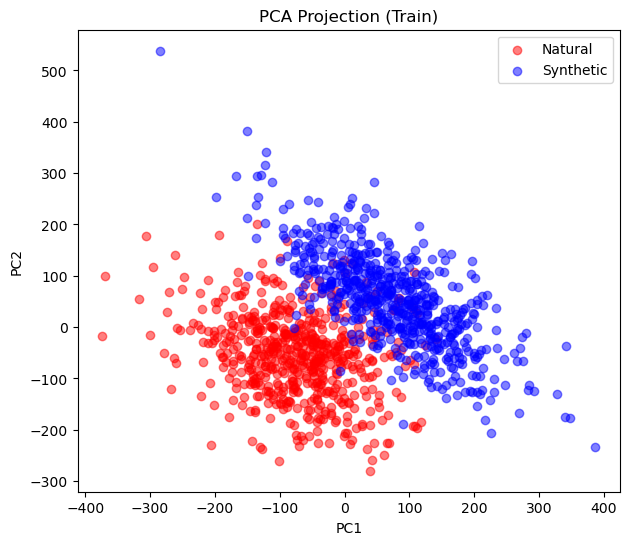
\includegraphics[width=\linewidth]{pca_train.png}
    \caption{Overall PCA behavior on the training responses.}
    \label{fig:pca-train}
  \end{subfigure}\hfill
  \begin{subfigure}[t]{0.47\linewidth}
    \centering
    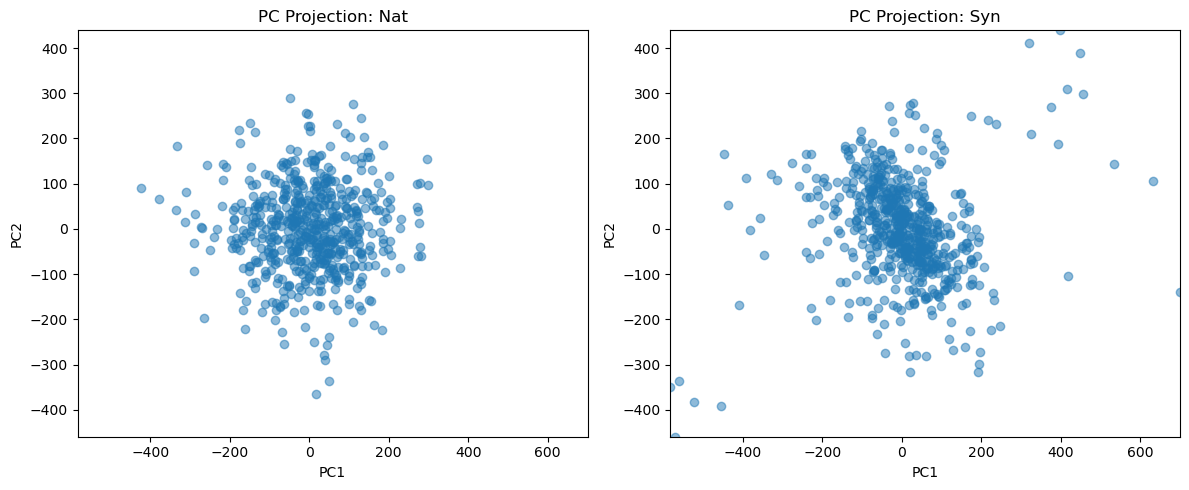
\includegraphics[width=\linewidth]{pca_conds.png}
    \caption{Condition-wise PCA structure for natural and synthetic trials.}
    \label{fig:pca-conds}
  \end{subfigure}
  \caption{PCA-based exploratory views of the masked fMRI response space.}
  \label{fig:pca-overview}
\end{figure}

The PCA projections indicate that class structure is not random in the leading neural dimensions. Natural and synthetic trials show partial geometric separation with overlap concentrated near the center of the plane. The condition-resolved view also suggests a dispersion difference, where one class forms a tighter cluster and the other is more diffuse, consistent with different levels of response consistency across trials.

Figure~\ref{fig:fa} shows stronger class mixing in FA space than in PCA space, indicating that dominant shared latent factors capture common variance rather than class-discriminative structure. In other words, FA emphasizes low-rank structure shared across conditions, while PCA preserves directions that are more useful for discrimination.

\begin{figure}[!htbp]
  \centering
  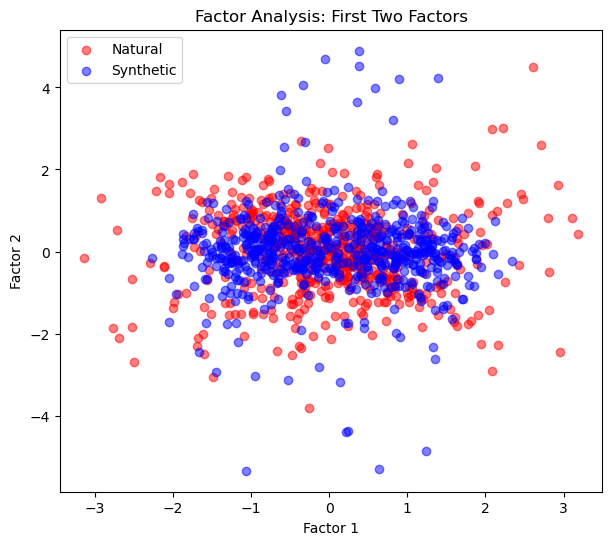
\includegraphics[width=0.75\linewidth]{fa.png}
  \caption{Factor-analysis visualization of shared latent structure in the masked fMRI responses.}
  \label{fig:fa}
\end{figure}

Together, these views support the decoder stage: condition signal is present, but concentrated in partially overlapping low-dimensional geometry rather than cleanly separable clusters.

\subsection*{Decoding with PCA Geometry Favors Linear Models}
Decoder performance is evaluated through PC-space error localization (Figure~\ref{fig:mlp-lr-pc}), confusion matrices (Figure~\ref{fig:mlp-lr-cm}), and training curves (Figure~\ref{fig:mlp-lr-s01}). This combination distinguishes geometric failure modes from aggregate class outcomes and optimization dynamics.

\begin{figure}[!htbp]
  \centering
  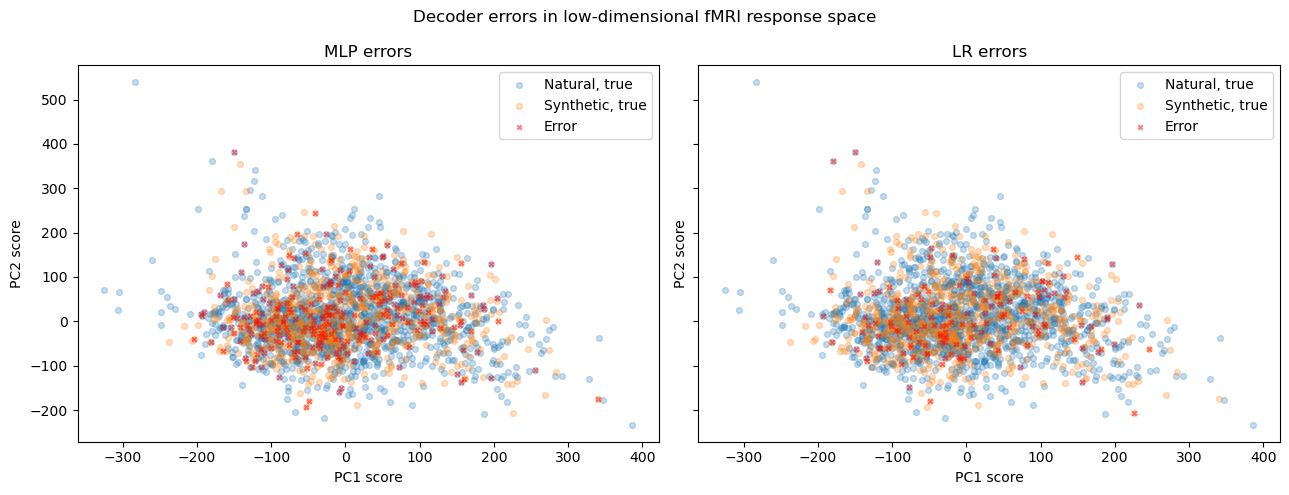
\includegraphics[width=0.64\linewidth]{mlp_vs_lr_pc.png}
  \caption{Error localization for MLP and logistic regression in the first two principal-component dimensions.}
  \label{fig:mlp-lr-pc}
\end{figure}

Figure~\ref{fig:mlp-lr-pc} shows that most errors cluster in the overlap region of PC1--PC2, consistent with intrinsic class mixing rather than isolated outlier failures. The logistic-regression panel exhibits fewer overlap-region errors than MLP, suggesting that a linear boundary is better aligned with the dominant discriminative axes in this reduced space.

\begin{figure}[!htbp]
  \centering
  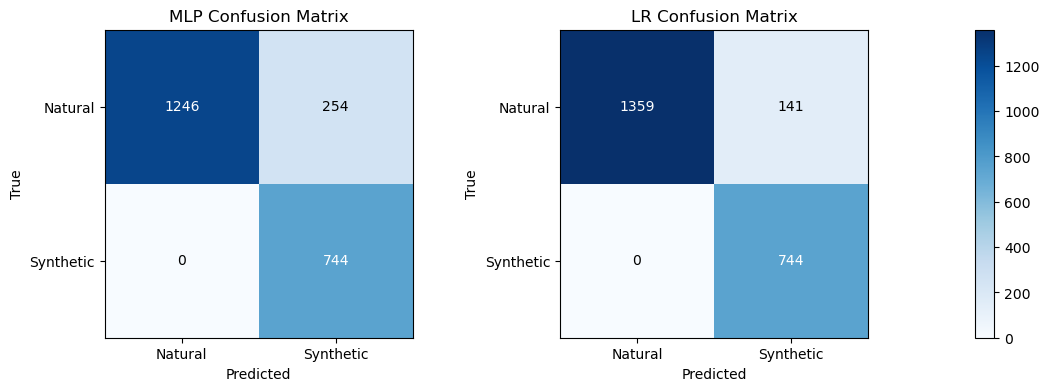
\includegraphics[width=0.64\linewidth]{mlp_vs_lr_cm.png}
  \caption{Confusion matrix comparison for MLP and logistic regression classifiers.}
  \label{fig:mlp-lr-cm}
\end{figure}

Figure~\ref{fig:mlp-lr-cm} quantifies the gap: logistic regression yields 2103/2244 correct predictions versus 1990/2244 for MLP. Both recover synthetic trials strongly (0 synthetic-to-natural errors), and the performance difference is driven by natural-to-synthetic overprediction (141 for logistic regression vs 254 for MLP). This asymmetric error pattern indicates that additional nonlinearity does not improve discrimination in the current representation and can increase false-positive synthetic calls.

Figure~\ref{fig:mlp-lr-s01} shows smoother MLP training loss, but this does not translate to better classification. Overall, decoder results indicate that linear boundaries are sufficient for most recoverable condition structure in the current PCA space, with remaining errors dominated by intrinsic overlap rather than model under-capacity.

\begin{figure}[!htbp]
  \centering
  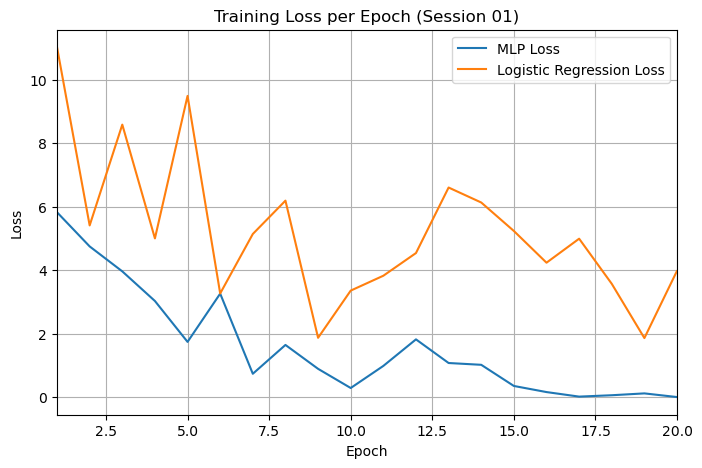
\includegraphics[width=0.64\linewidth]{mlp_vs_lr_s01.png}
  \caption{Subject-level comparison between MLP and logistic regression (subject 01).}
  \label{fig:mlp-lr-s01}
\end{figure}

\FloatBarrier

\subsection*{CNN Feature Geometry Shows Partial Alignment With Neural Structure}
Encoder analysis tests whether compact CNN features preserve structure predictive of neural PCs and whether this feature space supports stable mapping back to neural principal components.

\begin{figure}[!htbp]
  \centering
  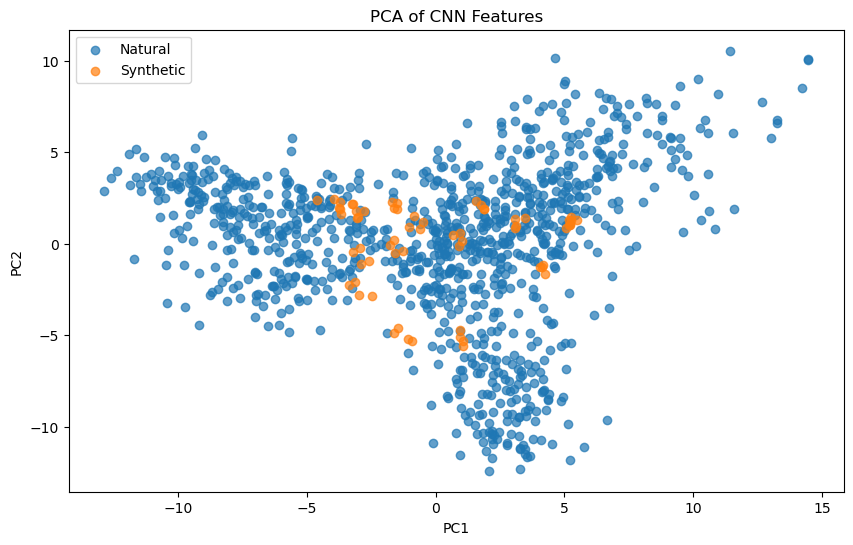
\includegraphics[width=0.78\linewidth]{pca_cnn.png}
  \caption{Low-dimensional structure of CNN-derived image features.}
  \label{fig:pca-cnn}
\end{figure}

In Figure~\ref{fig:pca-cnn}, synthetic samples occupy a compact region within a broader natural-image cloud, suggesting partial overlap in feature space but reduced coverage of natural-scene variability. This geometry implies that shared low-level feature axes are present, but the synthetic set does not span the full diversity of natural-scene structure.

\FloatBarrier

\subsection*{Ridge Regression Is the Most Reliable Encoder Across Neural Components}
The model comparison is summarized in Figure~\ref{fig:pc-encoders} (predicted-versus-actual values for the first three PCs) and Figure~\ref{fig:r2-encoders} (per-component $R^2$ across all 100 neural PCs).

\begin{figure}[!htbp]
  \centering
  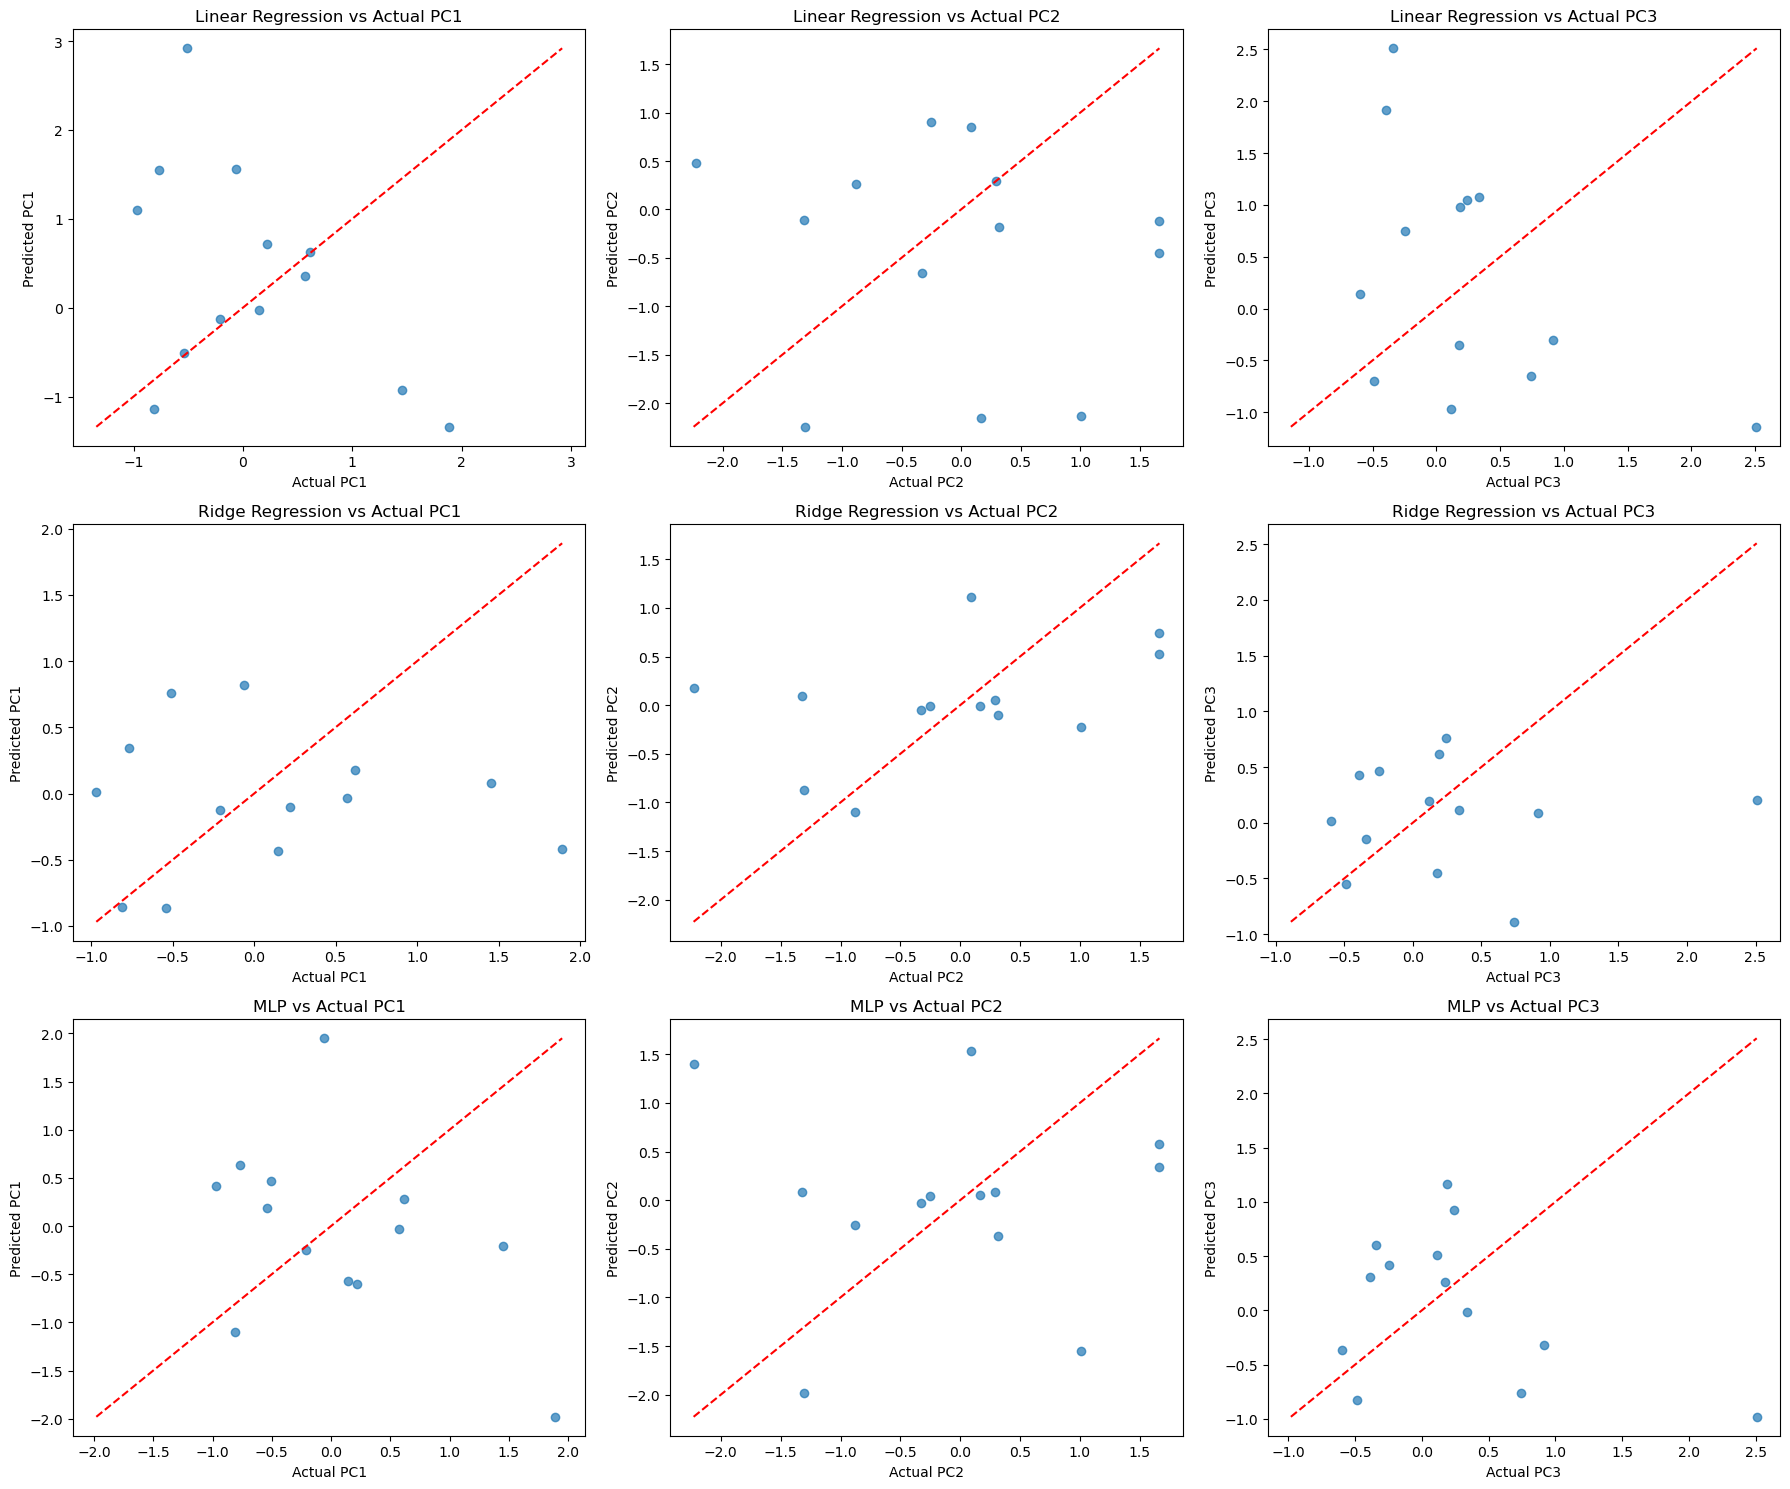
\includegraphics[width=0.76\linewidth]{pc_encoders.png}
  \caption{Predicted-versus-actual comparison for linear, ridge, and MLP encoders on the leading neural principal components.}
  \label{fig:pc-encoders}
\end{figure}

\begin{figure}[!htbp]
  \centering
  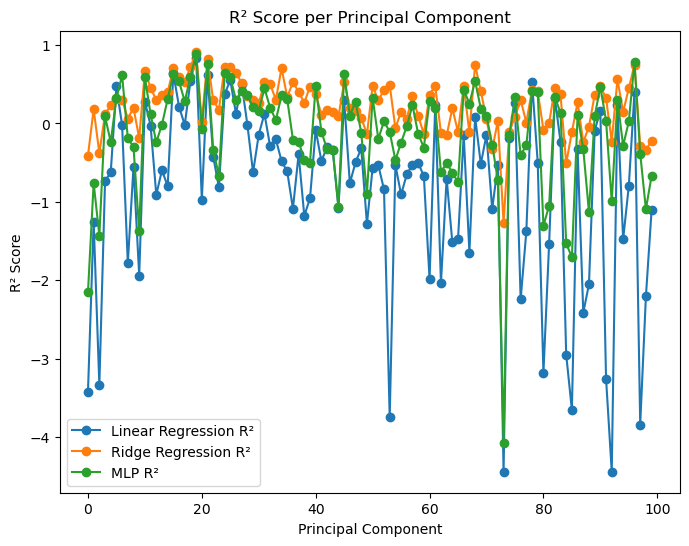
\includegraphics[width=0.76\linewidth]{r2_encoders.png}
  \caption{Per-component $R^2$ comparison across all 100 neural principal components.}
  \label{fig:r2-encoders}
\end{figure}

Figure~\ref{fig:pc-encoders} and Figure~\ref{fig:r2-encoders} both favor ridge: predictions are closer to diagonal for leading PCs and $R^2$ is more stable across components. Mean $R^2$ values are $-0.8506$ (linear), $0.2276$ (ridge), and $-0.1505$ (MLP), confirming ridge as the best encoder under limited paired samples.

Negative mean $R^2$ for linear regression and MLP indicates performance below a mean-predictor baseline on average across components, while ridge remains positive and comparatively stable. This supports ridge regularization as the strongest bias-variance tradeoff in the current small-sample encoder regime.

\FloatBarrier
\section{Discussion}
Results from both decoder and encoder analyses indicate that meaningful condition information is preserved in reduced neural space, and that regularized linear models are strong baselines in this regime. Logistic regression matched the low-dimensional geometry of the decoder task, while ridge regression provided the most stable encoding behavior across neural components.

The findings should be interpreted with key constraints in mind: pooled labels are imbalanced (natural $n=1500$ vs synthetic $n=744$), development is effectively single-subject/session-centered, and model selection was limited by compute and memory budgets. Future work should prioritize balanced multi-subject protocols and higher-capacity mappings (e.g., transformer-based feature extractors and cross-attention decoders) to test which image-to-neural relationships generalize beyond this within-subject baseline.

\section{Conclusion}
An end-to-end pipeline was developed to study neural decoding and encoding of natural versus synthetic visual stimuli using NSD/NSD-Synthetic responses. Across exploratory analyses, decoder evaluation, and encoder modeling, the results converged on a consistent finding: useful discriminative structure is present in low-dimensional neural representations, and simple regularized models capture that structure more reliably than higher-capacity alternatives in the current data regime. In decoding, logistic regression aligned well with PCA geometry and outperformed the MLP in pooled confusion-matrix behavior, indicating that most remaining errors are attributable to intrinsic class overlap rather than insufficient nonlinear capacity. In encoding, ridge regression achieved the strongest and most stable reconstruction profile across principal components, including the highest mean $R^2$, supporting regularization as a key requirement for small-sample image-to-neural mapping.

At the same time, conclusions are bounded by class imbalance, single-subject development, and computational constraints that limited model scale and search depth. The framework therefore serves as a reproducible baseline rather than a final account of biological visual computation. Future work should extend to balanced multi-subject protocols and higher-capacity transformer-based mappings from raw or high-dimensional image features to neural response space, with stronger uncertainty and stability analysis to test which representational relationships generalize robustly across subjects and conditions.

\section{Author Contributions}
I independently designed the project, implemented preprocessing and modeling pipelines, performed analyses, produced visualizations, interpreted results, and wrote the manuscript.

\section{Acknowledgments}
This project used data from the Natural Scenes Dataset (NSD) and the NSD-Synthetic extension. Development and analysis were supported by open-source scientific computing software, including NumPy, PyTorch, Matplotlib, and related Python tools. Consultation with Codex supported exploration of alternative memory-efficient PCA approaches and debugging during pipeline development, and ChatGPT was used for LaTeX compilation assistance. Thanks are also given to NeuroDong (GitHub) for sharing the NeurIPS LaTeX template setup used as a starting point. Helpful course guidance and discussions in CSE 599 also informed model design and interpretation.

% 中：引用格式全文一致；本示例 natbib + BibTeX（pdflatex → bibtex → pdflatex×2）。与 natbib 冲突时可用 \usepackage[nonatbib]{neurips_2026}，并在加载样式前 \PassOptionsToPackage{...}{natbib}（若仍用 natbib）。
% EN: One consistent style; this example uses natbib + BibTeX. If natbib clashes, use \texttt{nonatbib} and \verb|\PassOptionsToPackage| before loading \texttt{neurips\_2026} when needed.
{\small
\bibliographystyle{plainnat}
\bibliography{references}
}

\end{document}
